\documentclass{article}
\usepackage{cite}
\usepackage{hyperref}
\usepackage{graphicx}
\usepackage[onehalfspacing]{setspace}
% \usepackage[bottom=1in, top=1in, left=1in, right=1in]{geometry}

\author{Charlie Gunn and Zach Minot}
\title{Crosshatch: A Web Application for Crossword Collaboration}

\begin{document}
\maketitle

\section{Motivation and Introduction}
\label{mot}
When doing a crossword puzzle from a physical newspaper, it is easy for a few people to gather around and work on solving it together.
This is because all of the clues are visible at once, so each person can scan around for clues they know the answer to. However, this technique
for crossword collaboration does not extend well into the digital world. Most major websites that host interactive crosswords only show a small subset of
clues at a time (e.g. The LA Times \cite{latcrossword}), forcing all collaborators to focus on the same small portion of the clues. In the authors' personal experience,
this is an inferior way to collaborate on a crossword: a lot of the fun of joint crosswords is rapidly going back and forth in different areas
of the grid, calling out newly discovered answers.

To solve this problem, this paper introduces Crosshatch: a web application for crossword collaboration. Crosshatch
allows multiple participants to work on the \textit{same} crossword from their own personal devices (in a way similar to document-sharing services,
but for crosswords instead of general documents). To make finding and solving crosswords easy, Crosshatch provides access to multiple free daily crosswords
from around the US (LA Times, Wall Street Journal, Universal, etc.) and features a convenient user interface for solving.

% enjoyment of crosswords
% crosswords are really fun to do together!
% this is easy in a paper newspaper, but really hard online since only one clue displays at once
% (paper newspaper does not scale to large amounts of people)
\newpage
\subsection{Related Work}
\label{relatedwork}
% - paper on collaborative editing. mention how our case is simpler
Crosshatch's core technological design relies on a specific piece of real-time systems technology: collaborative editing.
Collaborative real-time editors are applications that enable seemingly instantaneous, simultaneous editing
of the same digital document by different users.
Possibly the most popular of collaborative editing tools is Google Docs \cite{googledocs}, a collaborative
word document tool similar to Microsoft Office Word.
The complex problem of creating a network structure to facilitate this type of application has been solved with centralized (Client/Server)
and P2P models \cite{p2p} \cite{p2p2}.
Furthermore, different protocols, such as push-based \cite{pushbased} or semi-synchronous \cite{semisynchronous}, can be implemented based on the type of information being edited,
network model constructed, and deadlines for edits to cascade through the network.

However, collaboration on a crossword is much simpler than collaboration on a text file; it requires only
single character inputs at designated points with no formatting or large edits. This eliminates the main challenge of collaborative editing,
which is contradictory edits which are non-trivial to merge (e.g., one user deletes the word ``beet'', while another inserts a `g' to make ``beget'').
Crosshatch does not have to deal with these sorts of issues due to the nature of single-character grid-based editing -- the server can perform edits in
exactly the order it receives them, with no issues. See Section \ref{editsharing} for more details.

\section{System Architecture}
\subsection{Basic Structure}

In designing Crosshatch, it was first important to decide what \textit{type} of application to create. When solving crosswords, the authors have the most
experience with smartphone apps (particularly, the New York Times Crossword App). However, going this route limits the app to a
specific platform, and the authors wanted to include as much extendability and scalability as possible. This
prompted the decision to create a web application. The authors also have considerably more experience in creating web applications
than in creating mobile apps, which reduced development time-cost significantly.

Crosshatch was built with four major system components: a frontend user interface, a backend server and API, a persistent database,
and a file storage mechanism.

The frontend library of choice was \textbf{Vue3}. This decision was mainly superficial -- the authors' wanted to try an updated, state-of-the-art library
that they had never used before. Vue3 also provides somewhat similar conceptual programming to React, which both authors have had experience with in the past.

For the backend, \textbf{FastAPI} was chosen due to its support and familiarity. The authors have had prior experience with FastAPI and Python backend APIs in general, so it was the default choice for the backend for this application.

\textbf{PostgresSQL} was chosen for the type of database for similar reasons to above, with the added benefit of scalability in the
future if this application were to extend beyond the scope of this class.

The file storage mechanism is temporarily hosted within the backend. This is acceptable for now due to the limited amount of crossword storage the platform needs;
however, in the future, this simple solution will likely need to be replaced with some sort of file storage server on the cloud, such as an S3 bucket.

The entire thing is packaged into a single docker-compose application with each of these services. The deployed version of Crosshatch is hosted on an AWS EC2 instance, and can be accessed at \url{http://54.205.97.70:8080/}.
\subsection{Edit Sharing}
\label{editsharing}

The collaborative crossword architecture was created using the websockets rooms functionality. With websockets, there are rooms,
or sessions, that clients can join and listen for events broadcasted to that specific room. In Crosshatch, a websocket room is created for each individual collaborative crossword, and clients are automatically subscribed to a room when they open the webpage associated with that crossword. Each time the crossword is edited,
a single character-change event is broadcasted to all other clients in that room, and both the server's and the clients' representations of the crossword are updated
to match the ground truth.

In Google Docs and other colaborative editing tools, text file edit conflicts can become extremely complex as stated in \ref{relatedwork}. However, Crosshatch eliminates all
editing conflicts due to the nature of of single character edits.
Essentially, crossword edits are \textbf{atomic}, and their locations are \textbf{statically determined} by nature, which allows Crosshatch to simply consume the edit events in order of reception without issue. As long as the server broadcasts each edit event before dequeueing the next one, synchronization is guaranteed.

\subsection{Crossword Ingestion}

Another core, but small, part of the application is the ingestion of free crosswords from newspapers. There is no official exposed service
that the authors could find for this functionality, save for a few websites that self host the \texttt{.puz} file representations of some major newspapers.
To achieve this, a script was written to scrape the website \url{crosswordfiend.com} and acquire some of the \texttt{.puz} files of the current day.
At the moment, this script must be manually run, but hopefully will eventually be automatically scheduled.

\section{Current Functionality and Workflow}

Crosshatch's main functionality is collaborative crossword editing. A user can create a crosshatch session, and then
share the link with others to add other users to the session. To choose a crossword for a session, a user can either choose one of the
already existing crosswords in the database, or upload and title their own crossword in the format of a \texttt{.puz} file. This uploaded \texttt{.puz} file is then added to the database
for all other users to utilize.

\begin{figure}[t]
  \centering
  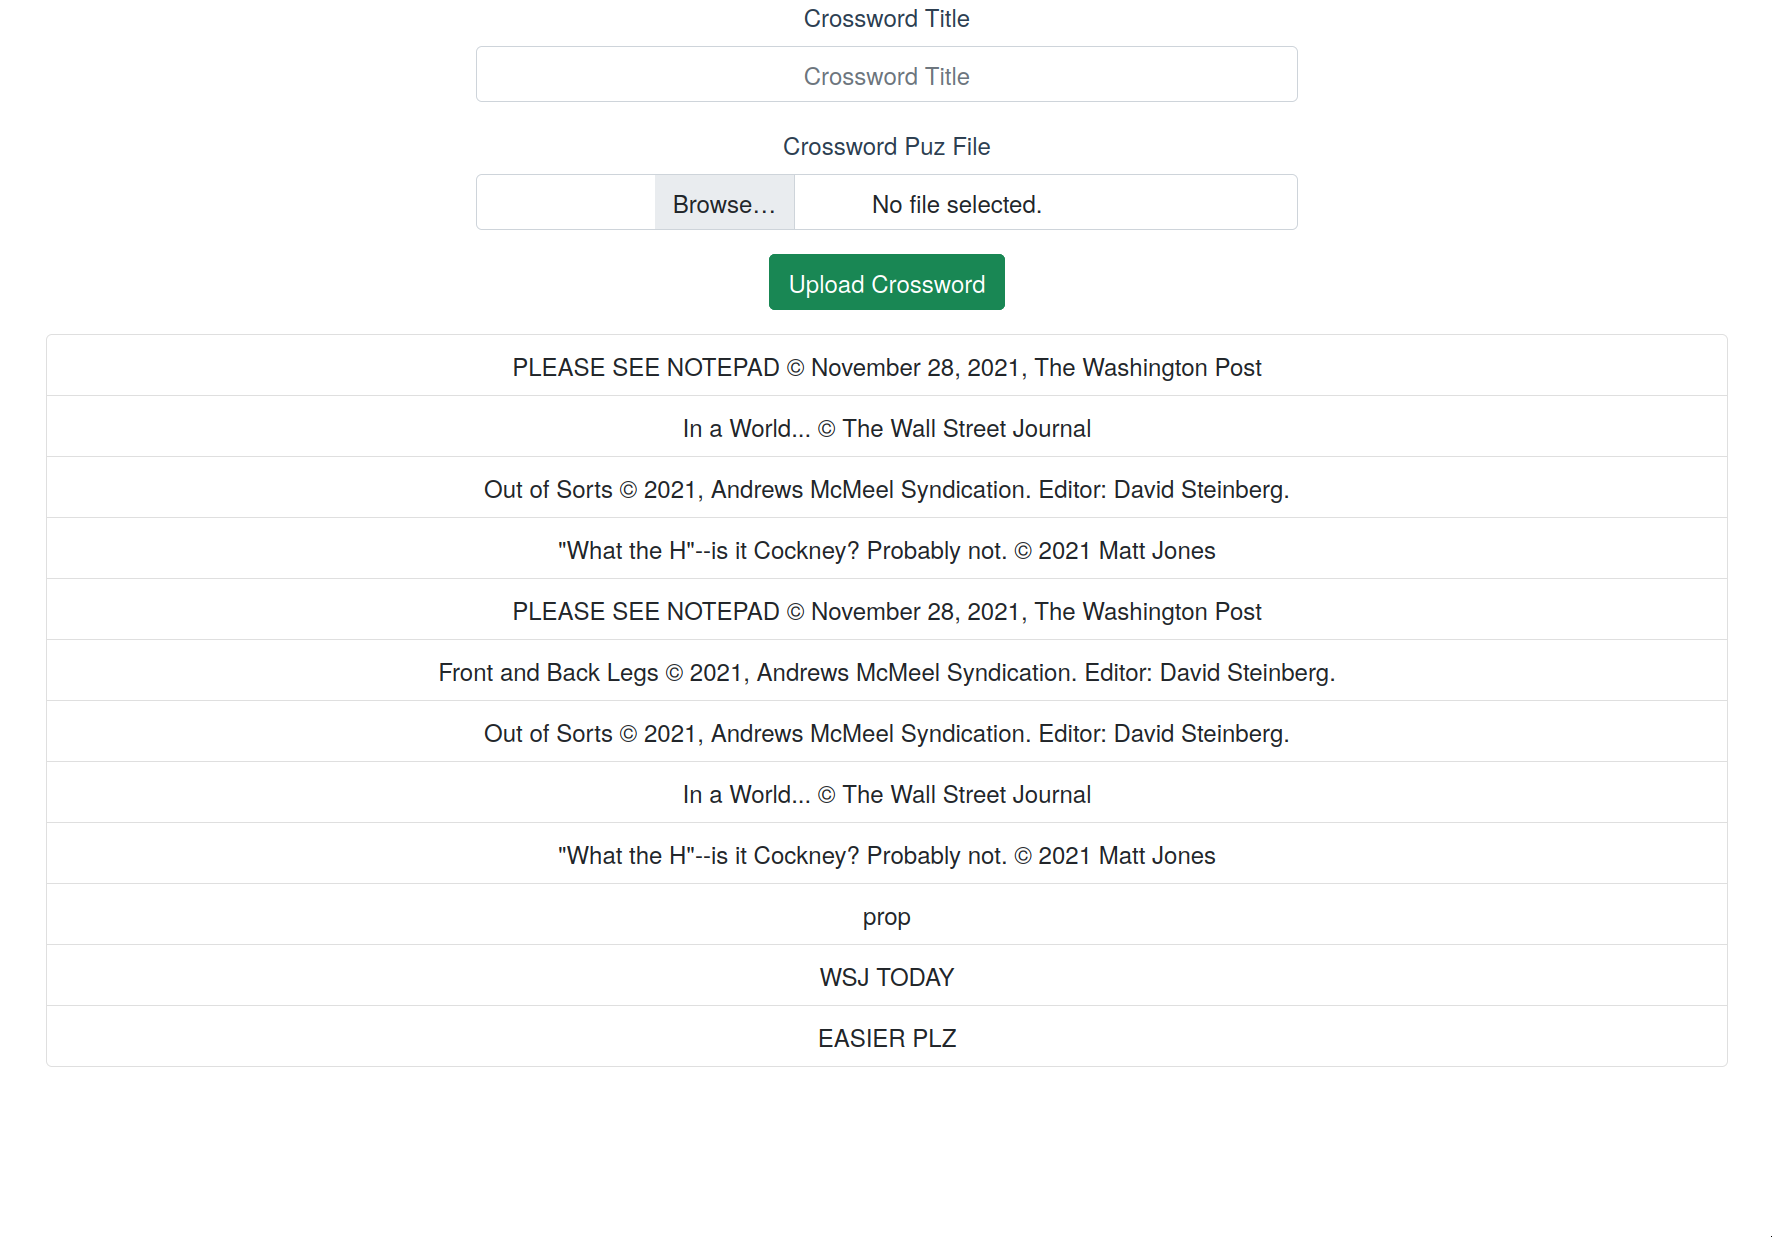
\includegraphics[width = \linewidth]{img/list.png}
  \caption{The main page of Crosshatch}
  \label{list}
\end{figure}
\begin{figure}[t]
  \centering
  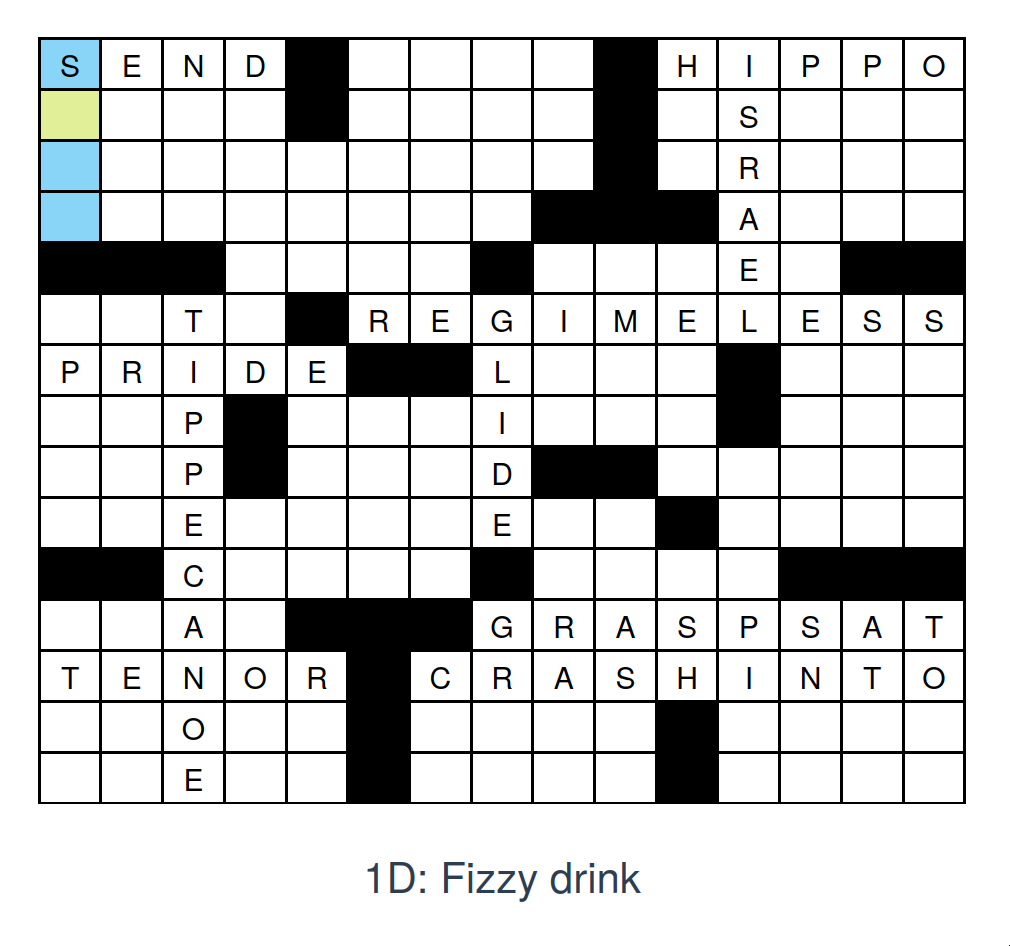
\includegraphics[width = \linewidth]{img/crossword.png}
  \caption{Crosshatch's crossword editing UI}
  \label{cross}
\end{figure}


% let's add some screenshots here
Crosshatch has two main screens: the puzzle select screen (see Figure \ref{list}) and the collaboration screen (see Figure \ref{cross}). The puzzle select screen includes the user interface for uploading a custom crossword
and selecting a crossword to create a session. To upload a custom crossword, the user needs to title the crossword in the input form, upload the \texttt{.puz} file representation of the crossword,
and click submit. After the user refreshes the page, they can see their crossword added to the list of current crosswords in the database. To select a crossword,
the user simply needs to click on the title of the crossword in the list and they will be redirected to their collaborative editing page.

The collaborative editing page showcases only the crossword and the current clue. The current row or column is highlighted on the crossword, and the corresponding clue
is shown below the crossword. At the most basic level, a user can click on a square to edit, and then type a character to place into the square. The user's cursor will
move to the next square in the current clue, or the next clue if there are no more squares in the current clue. Pressing backspace will delete the character from the current square,
and move the cursor or clue backwards similarly.

The editing page also offers a set of keyboard controls. The arrow keys will change the clue from across to down or move the cursor in the coresponding direction. Space will
switch the clue from across to down and vice versa. Delete removes the current letter, but does not move the cursor backwards. Tab will move forward one clue,
while Shift + Tab will move backwards one clue. This closely replicates the keyboard interface of the online NYT crossword.

Finally, to collaborate with a friend, all one needs to do is \textit{copy} the URL of their collaborative crossword session and send it. Anyone who goes to that link will be able to simultaneously collaborate on the crossword in real-time!

\section{Future Work}
There are many possibly directions for future work, since there 
are many additional features that would be useful in a crossword editing application. 
A few possibilities are listed below:
\begin{itemize}
	\item Optional incorrect character detection
  	\item UI customization (increase crossword size, add colors to letter inputs, customize controls, etc.)
	\item Adding a save-and-quit feature
	\item Adding a chat function
\end{itemize}

\section{Conclusion}
Ultimately, we are very proud of the state that Crosshatch is in, and learned a lot about many different technologies and aspects of software development as we created it. Hopefully we will be able to continue this project in the future to create a more complete application... we already bought a dedicated domain for it!



\newpage
\bibliography{sources.bib}
\bibliographystyle{plain}

\end{document}
